\documentclass[oneside,12pt,openany]{report}

% ======================================================================
%  TIET report layout (built in, so no external tietreport.cls is needed)
% ======================================================================
\makeatletter
%% ===================================================
%% Geometry: Page margins (same on every page)
%% ===================================================
%% Equal left and right margins keep the 6in text
%% block in the same place on every page and centre
%% the title page. Top/bottom margins accommodate
%% headers/footers and content balance.
\usepackage[
  left=1.25in,
  right=1.25in,
  top=1.8in,
  bottom=0.85in
]{geometry}

%% ===================================================
%% Fancyhdr: Headers with page numbers
%% ===================================================
%% All pages: page number + course header on the
%% left. Footer empty to maximize text area.
%% Header rule (0.5pt) provides visual separation.
\usepackage{fancyhdr}
\pagestyle{fancy}
\fancyhf{}
\fancyhead[L]{\thepage \quad \@tpHeader}
\renewcommand{\headrulewidth}{0.5pt}
\renewcommand{\footrulewidth}{0pt}

%% ===================================================
%% Titlesec: Custom chapter title formatting
%% ===================================================
%% Chapter titles use raggedleft (right-aligned)
%% with bold/large label, followed by huge title
%% and horizontal rule. Spacing optimized for
%% visual hierarchy. Chapter opening pages use
%% empty style (no headers).
\usepackage{titlesec}
\titleformat{\chapter}[display]
  {\raggedleft\bfseries\large}
  {Chapter \thechapter}
  {0.3em}
  {\huge}
  [\vspace{0.1em}\hrule]
\titlespacing*{\chapter}{0pt}{-50pt}{40pt}
\assignpagestyle{\chapter}{empty}

%% ===================================================
%% Required packages: Hyperref, graphics, math
%% ===================================================
%% Standard packages for links, images, and
%% mathematical notation support.
\usepackage{hyperref}
\usepackage{graphicx}
\usepackage{amsmath}
\usepackage{amssymb}

%% ===================================================
%% Internal Variables: Title page content storage
%% ===================================================
%% Prefix @tp denotes "title page" internal vars.
%% These hold configuration set via public commands
%% below. Users should not access these directly.

%% Title page header (e.g., course code and lab)
\newcommand{\@tpHeader}{%
  UCS 503 Software Engineering Project Report%
}

%% Main project title
\newcommand{\@tpTitle}{Proposal to Final}

%% Project subtitle/description
\newcommand{\@tpSubTitle}{%
  How to Write a Project Report%
}

%% Author list (4 students with roll numbers)
\newcommand{\@tpAuthors}{%
  \texttt{102XXXXXXX} {Name Title} \\
  \texttt{102XXXXXXX} {Name Title} \\
  \texttt{102XXXXXXX} {Name Title} \\
  \texttt{102XXXXXXX} {Name Title}%
}

%% Degree, year, group info below authors
\newcommand{\@tpSubText}{%
  Group: \texttt{3XXX} BE Third Year, CSE%
}

%% Faculty advisor/guide name
\newcommand{\@tpAdvisor}{%
  Dr. NAME OF THE ADVISOR%
}

%% Footer: evaluation period, department, institution
\newcommand{\@tpFooter}{%
  \large Mid-Semester Evaluation \\[0.2cm]
  \bfseries Computer Science and Engineering%
  \\ Department \\[0.15cm]
  Thapar Institute of Engineering and%
  \\ Technology, Patiala%
}

%% ===================================================
%% Public Commands: User-facing configuration
%% ===================================================
%% Call these in preamble to customize title page.
%% Example: \TitlePageHeader{CS 504 Lab}

%% Set title page header
\newcommand{\TitlePageHeader}[1]{%
  \renewcommand{\@tpHeader}{#1}%
}

%% Set main project title
\newcommand{\ProjectTitle}[1]{%
  \renewcommand{\@tpTitle}{#1}%
}

%% Set project subtitle
\newcommand{\ProjectSubTitle}[1]{%
  \renewcommand{\@tpSubTitle}{#1}%
}

%% Set author list (override default)
\renewcommand{\author}[1]{%
  \renewcommand{\@tpAuthors}{#1}%
}

%% Set degree/year/group info
\newcommand{\TitlePageSubText}[1]{%
  \renewcommand{\@tpSubText}{#1}%
}

%% Set advisor name
\newcommand{\AdvisorName}[1]{%
  \renewcommand{\@tpAdvisor}{#1}%
}

%% Set footer text (evaluation period, dept, etc)
\newcommand{\TitlePageFooterText}[1]{%
  \renewcommand{\@tpFooter}{#1}%
}

%% ===================================================
%% Maketitle: Render custom title page
%% ===================================================
%% Override \maketitle to produce styled title page
%% using configured variables. Centered layout with
%% institutional branding. After title page, a blank
%% page follows (ready for TOC on next page).

\renewcommand{\maketitle}{%
  \begin{titlepage}
    \thispagestyle{empty}
    \centering
    \vspace*{0.5cm}

    {\large \textbf{\@tpHeader}}

    \vspace{2cm}
    {\LARGE \textbf{\@tpTitle}}

    \vspace{0.2cm}
    {\@tpSubTitle}

    \vspace{3.5cm}
    {\large \textbf{Submitted by:}}

    \vspace{0.2cm}
    {\large \@tpAuthors}

    \vspace{0.5cm}
    {\normalsize \@tpSubText}

    \vfill

    {\large \textbf{Submitted to:}}

    \vspace{0.2cm}
    {\normalsize \@tpAdvisor}

    \vspace{2cm}
    {\normalsize \@tpFooter}
  \end{titlepage}

  \newpage
  \thispagestyle{empty}%
}
\makeatother



% Extra packages required by the report content
\usepackage{float}
\usepackage{tabularx}
\usepackage{xcolor}
\usepackage{listings}
\usepackage{adjustbox}
\usepackage{needspace}
\usepackage{tikz}
\usetikzlibrary{arrows.meta,positioning,shapes.geometric,fit,calc}



%% ==================================================
%% CODE LISTING AND DIAGRAM STYLES
%% ==================================================

\lstdefinestyle{code}{
  basicstyle=\ttfamily\scriptsize,
  keywordstyle=\bfseries,
  commentstyle=\color{gray}\itshape,
  numbers=left, numberstyle=\tiny\color{gray}, numbersep=5pt,
  frame=single, rulecolor=\color{gray!60},
  backgroundcolor=\color{gray!6},
  breaklines=true, tabsize=2, showstringspaces=false,
  xleftmargin=1.2em, aboveskip=4pt, belowskip=2pt
}
\lstdefinelanguage{json}{
  string=[b]", morekeywords={true,false}, sensitive=true
}

\tikzset{
  >=Stealth,
  blk/.style={rectangle,rounded corners=3pt,draw=black,fill=white,thick,
              minimum height=1.2cm,text width=2.3cm,align=center,font=\small},
  fl/.style={font=\scriptsize,align=center}
}

% ground symbol: \gnd{coordinate}
\newcommand{\gnd}[1]{%
  \draw[thick] (#1) -- ++(0,-0.3) coordinate (g);
  \draw[thick] ($(g)+(-0.25,0)$) -- ($(g)+(0.25,0)$);
  \draw[thick] ($(g)+(-0.16,-0.08)$) -- ($(g)+(0.16,-0.08)$);
  \draw[thick] ($(g)+(-0.07,-0.16)$) -- ($(g)+(0.07,-0.16)$);}

% UML stick-figure actor: \actor{x}{y}{label}
\newcommand{\actor}[3]{%
  \begin{scope}[shift={(#1,#2)}]
    \draw[thick] (0,0.55) circle (0.17);
    \draw[thick] (0,0.38)--(0,-0.1) (-0.3,0.25)--(0.3,0.25)
                 (0,-0.1)--(-0.25,-0.5) (0,-0.1)--(0.25,-0.5);
    \node[font=\footnotesize,align=center,below] at (0,-0.5) {#3};
  \end{scope}}

% Scale a diagram down only if it is wider/taller than the page allows
\newcommand{\fitfig}[2][0.27]{\begin{adjustbox}{max width=\linewidth,max height=#1\textheight,center}#2\end{adjustbox}}

%% ==================================================
%% CUSTOMIZE THESE FIELDS FOR YOUR PROJECT
%% ==================================================

% Course/Lab header
\TitlePageHeader{%
  UCS 503 - Software Engineering%
}

% Main project title
\ProjectTitle{%
  SmartLib: Library Seat Allocator%
}

% Subtitle or project description
\ProjectSubTitle{%
  An IoT System for Real-Time Seat Monitoring and Management%
}

% Student information (up to 4 students)
\author{%
  \texttt{1024031135} Saksham Kansal \\
  \texttt{1024031118} Ishaan Gupta \\
  \texttt{1024031137} Sanshi%
}

% Group number, degree, year, program
\TitlePageSubText{%
  Computer Engineering Department (COE)%
}

% Faculty advisor/guide name
\AdvisorName{%
  Ms. Jhonsy Bansal%
}

% Evaluation period and department info
\TitlePageFooterText{{%
    \large November 2026 \\[0.2cm]
    \bfseries Computer Engineering
    Department%
  } \\[0.15cm]
  Thapar Institute of Engineering and Technology,
  Patiala%
}

%% ==================================================

\begin{document}

% Let partly filled pages end early instead of stretching the spacing
\raggedbottom

% Generate title page
\maketitle

% Table of contents (auto-generated from chapters)
\tableofcontents

% ===== CHAPTER 1: INTRODUCTION =====

\chapter{Introduction}

\section{Background and Context}

University libraries are busiest during exams and assignment deadlines. At these times,
users have to walk through the reading halls to find a free seat. Gate counters show how many
people are inside, but not \emph{where} the free seats are. This wastes time and creates noise
that disturbs people who are studying.

Low-cost Wi-Fi boards, simple sensors and real-time cloud databases now make it possible to
track every seat and show its status on any phone or screen within a second.

\subsection{Problem Statement}
\label{sec:problem}

Finding a seat today has three main problems, listed in Table~\ref{tab:problems}.

\begin{table}[H]
\centering
\small
\renewcommand{\arraystretch}{1.1}
\begin{tabularx}{\linewidth}{|>{\raggedright\arraybackslash}p{0.2\linewidth}|>{\raggedright\arraybackslash}X|>{\raggedright\arraybackslash}p{0.27\linewidth}|}
  \hline
  \textbf{Problem} & \textbf{Description} & \textbf{What is needed} \\
  \hline
  Manual search &
  Users walk across floors and aisles at busy times, which wastes time and creates noise. &
  A way to see free seats before walking to the hall. \\
  \hline
  No seat-level view &
  Headcount boards at the gate show only a total count, not which desks are free. &
  Status of each seat instead of one building-wide number. \\
  \hline
  No data for staff &
  Staff have no live or past usage data to spread users across halls or plan facilities
  such as cooling. &
  Live and past usage reports for planning. \\
  \hline
\end{tabularx}
\caption{Main problems and what is needed}
\label{tab:problems}
\end{table}

\section{Project Objectives}

\begin{enumerate}
  \item \textbf{Detection:} Detect whether each seat is in use with low-cost IR sensors.
  \item \textbf{Noise filtering:} Ignore short disturbances, such as a passing hand, so a
    seat's status does not flicker.
  \item \textbf{Transmission:} Send seat status to the cloud over Wi-Fi with little delay.
  \item \textbf{User view:} Show a live seat map and seat counts on phones and on a screen at
    the entrance.
  \item \textbf{Admin view:} Give staff a dashboard with usage, session time and busy hours.
  \item \textbf{Reservations:} Let a user hold a seat for a short time, either with the push
    button at the desk or with an ID card at the entrance kiosk.
  \item \textbf{Usage history:} Record each sitting as a session so that past usage can be
    shown as charts.
  \item \textbf{Opening hours:} Let staff set the library timings, and stop reservations and
    show seats as closed outside them.
\end{enumerate}

\subsection{Scope and Organisation of the Report}

The system covers sensing, sending, storing and displaying seat status for one library zone,
together with short seat reservations, usage history and opening hours. It only detects
whether a seat is in use. It does not take pictures or track people; the only personal data
kept is the roll number used for a kiosk reservation. The final system shows the full path
from a sensor to a web browser for three monitored seats, and more seats or zones can be added
with more sensor nodes and database entries.

Chapter~\ref{ch:method} covers the requirements, development model, design, diagrams and
implementation. Chapter~\ref{ch:results} gives the test plan and limitations, and
Chapter~\ref{ch:concl} concludes with future work.

% ===== CHAPTER 2: METHODOLOGY & DESIGN =====

\chapter{Methodology and Design}
\label{ch:method}

\section{Requirements Analysis}
\label{sec:req}

\subsection{Stakeholders}

\begin{itemize}
  \item \textbf{Users:} Want to know which seats are free and how full the library is.
  \item \textbf{Library staff / administrators:} Want live and past usage data to manage
    the library.
  \item \textbf{Sensor node (system actor):} Checks each seat and sends its status. It is the
    only part of the system that writes seat values.
  \item \textbf{Session recorder (system actor):} A small background program that watches
    the seat values and saves each sitting as a session for the usage charts.
\end{itemize}

\subsection{Functional Requirements}

\begin{table}[H]
\centering
\small
\renewcommand{\arraystretch}{1.1}
\begin{tabularx}{\linewidth}{|l|>{\raggedright\arraybackslash}X|}
  \hline
  \textbf{ID} & \textbf{Requirement} \\
  \hline
  FR1 & Detect whether a person is at each seat using an IR sensor. \\
  \hline
  FR2 & Change a seat between free and taken only after the reading stays the same for
        5~seconds (debounce). \\
  \hline
  FR3 & Send one value per seat to the cloud: 0 free, 1 taken, 2 reserved. \\
  \hline
  FR4 & Show a live seat map and seat counts on all screens without a page refresh. \\
  \hline
  FR5 & Holding a seat's push button for 3~seconds reserves it for 60~seconds. \\
  \hline
  FR6 & Let a user reserve a free seat at the kiosk for 1~minute, one at a time; the hold
        ends when the seat becomes taken. \\
  \hline
  FR7 & Save each sitting as a session and show usage charts to staff. \\
  \hline
  FR8 & Stop reservations and show seats as closed outside the opening hours set by
        staff. \\
  \hline
\end{tabularx}
\caption{Functional requirements}
\label{tab:fr}
\end{table}

\subsection{Non-Functional Requirements}

\begin{table}[H]
\centering
\small
\renewcommand{\arraystretch}{1.1}
\begin{tabularx}{\linewidth}{|l|l|>{\raggedright\arraybackslash}X|}
  \hline
  \textbf{ID} & \textbf{Attribute} & \textbf{Requirement} \\
  \hline
  NFR1 & Performance & Screens update within one second of a database change (not counting
                       the 5-second debounce). \\
  \hline
  NFR2 & Reliability & Short disturbances must not make seat colours flicker. \\
  \hline
  NFR3 & Usability   & The user interface works well on a phone, tablet and kiosk screen. \\
  \hline
  NFR4 & Security    & Only the ESP32 can write seat values, and only signed-in staff can
                       open the admin dashboard. \\
  \hline
  NFR5 & Cost        & Uses cheap hardware and runs on the free Firebase plan. \\
  \hline
\end{tabularx}
\caption{Non-functional requirements}
\label{tab:nfr}
\end{table}

\section{Software Development Process Model}
\label{sec:process}

The project follows the \emph{Incremental Development Model}~\cite{sommerville,pressman}.
The requirements in Section~\ref{sec:req} are set first. The system is then built in parts
(increments). Each part is designed, built and tested, then joined to the parts already
finished, so every stage ends with something that works (Figure~\ref{fig:process}).

\begin{figure}[H]
\centering
\fitfig[0.3]{%
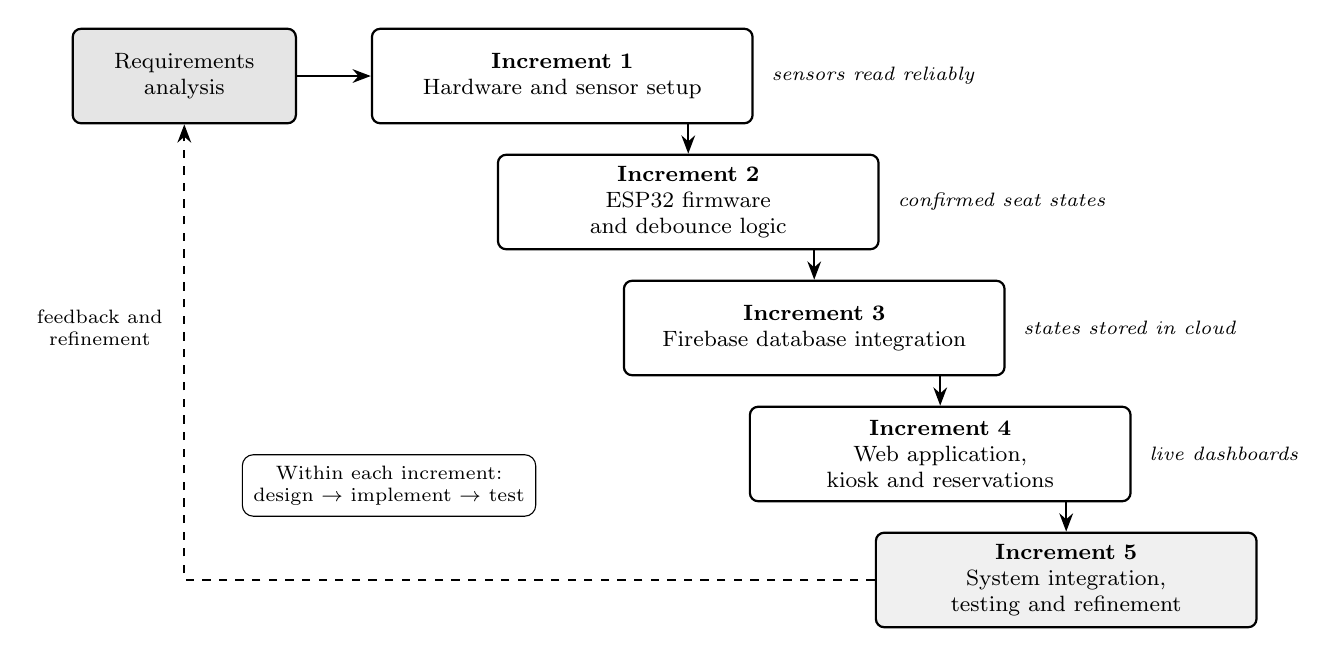
\begin{tikzpicture}[
  req/.style={rectangle,rounded corners=3pt,draw,thick,fill=gray!20,minimum height=1.2cm,
              text width=2.6cm,align=center,font=\footnotesize},
  inc/.style={rectangle,rounded corners=3pt,draw,thick,fill=white,minimum height=1.2cm,
              text width=4.6cm,align=center,font=\footnotesize},
  incout/.style={font=\scriptsize\itshape,align=left,anchor=west}]
  \node[req] (r)  at (0,0) {Requirements\\analysis};
  \node[inc] (i1) at (4.8,0)     {\textbf{Increment 1}\\Hardware and sensor setup};
  \node[inc] (i2) at (6.4,-1.6)  {\textbf{Increment 2}\\ESP32 firmware and debounce logic};
  \node[inc] (i3) at (8.0,-3.2)  {\textbf{Increment 3}\\Firebase database integration};
  \node[inc] (i4) at (9.6,-4.8)  {\textbf{Increment 4}\\Web application, kiosk and reservations};
  \node[inc,fill=gray!12] (i5) at (11.2,-6.4) {\textbf{Increment 5}\\System integration,
                                               testing and refinement};
  \draw[->,thick] (r) -- (i1);
  \draw[->,thick] (i2.north |- i1.south) -- (i2.north);
  \draw[->,thick] (i3.north |- i2.south) -- (i3.north);
  \draw[->,thick] (i4.north |- i3.south) -- (i4.north);
  \draw[->,thick] (i5.north |- i4.south) -- (i5.north);
  \node[incout] at ([xshift=3pt]i1.east) {sensors read reliably};
  \node[incout] at ([xshift=3pt]i2.east) {confirmed seat states};
  \node[incout] at ([xshift=3pt]i3.east) {states stored in cloud};
  \node[incout] at ([xshift=3pt]i4.east) {live dashboards};
  \draw[->,thick,dashed] (i5.west) -| (r.south);
  \node[fl,anchor=east] at (-0.15,-3.2) {feedback and\\refinement};
  \node[draw,rounded corners,font=\scriptsize,align=center,inner sep=4pt] at (2.6,-5.2)
       {Within each increment:\\design $\rightarrow$ implement $\rightarrow$ test};
\end{tikzpicture}}
\caption{Incremental development model for the Library Seat Allocator}
\label{fig:process}
\end{figure}

Increment 1 fits the IR sensors and push buttons to the ESP32 and checks their output at
each seat. Increment 2 adds sensor reading, the 5-second debounce and the 60-second button
reservation (FR1, FR2, FR5). Increment 3 sends the seat values to Firebase (FR3, FR4).
Increment 4 builds the user dashboard, admin dashboard, entrance kiosk, kiosk reservations,
session recording and opening hours (FR4, FR6--FR8). Increment 5 joins everything,
puts the web app online and tests it with the cases in Chapter~\ref{ch:results}; any problems
are fixed in the earlier parts.

\textbf{Why this model.} The project has hardware, firmware, a cloud database and a web app,
and each part depends on the one before it. Building them one at a time lets each part be
tested on its own, so a fault is easy to locate. Each increment also gives a working result
that can be shown, and later parts can change without starting over.

\section{System Architecture}

\subsection{High-Level Design}

The system has three layers (Figure~\ref{fig:arch}): the \emph{edge layer} senses the seats,
the \emph{cloud layer} stores and shares their status, and the \emph{presentation layer}
shows it to users and staff. A small \emph{session recorder} runs on a library computer and
turns the live seat values into usage history.

\begin{figure}[H]
\centering
\fitfig{%
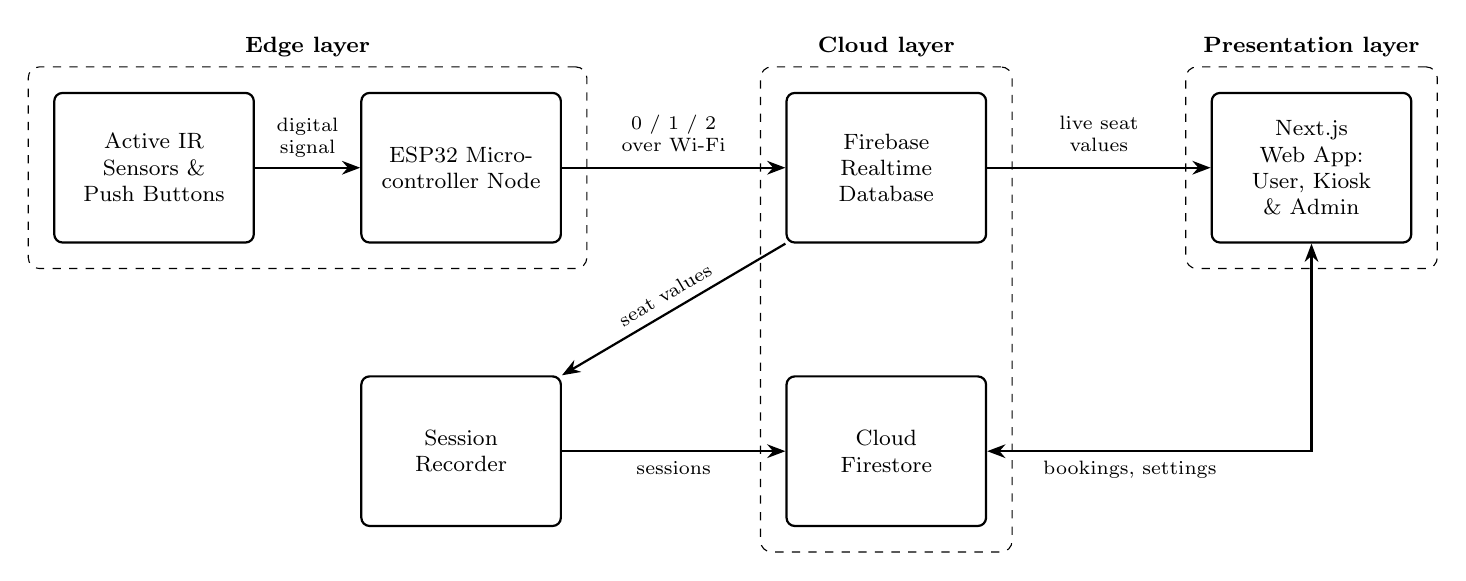
\begin{tikzpicture}[blk/.append style={text width=2.3cm,minimum height=1.9cm,font=\footnotesize}]
  \node[blk] (ir)  at (0,0)    {Active IR Sensors \&\\Push Buttons};
  \node[blk] (esp) at (3.9,0)  {ESP32 Micro-controller Node};
  \node[blk] (fb)  at (9.3,0)  {Firebase\\Realtime Database};
  \node[blk] (fs)  at (9.3,-3.6) {Cloud\\Firestore};
  \node[blk] (web) at (14.7,0) {Next.js Web App:\\User, Kiosk \& Admin};
  \node[blk] (rec) at (3.9,-3.6) {Session\\Recorder};
  \node[draw=black,dashed,rounded corners,fit=(ir)(esp),inner sep=9pt,
        label={[font=\footnotesize\bfseries,text=black]above:Edge layer}] (edge) {};
  \node[draw=black,dashed,rounded corners,fit=(fb)(fs),inner sep=9pt,
        label={[font=\footnotesize\bfseries,text=black]above:Cloud layer}] (cloud) {};
  \node[draw=black,dashed,rounded corners,fit=(web),inner sep=9pt,
        label={[font=\footnotesize\bfseries,text=black]above:Presentation layer}] (pres) {};
  \draw[->,thick] (ir)  -- node[fl,above]{digital\\signal} (esp);
  \draw[->,thick] (esp) -- node[fl,above=2pt]{0 / 1 / 2\\over Wi-Fi} (fb);
  \draw[->,thick] (fb)  -- node[fl,above=2pt]{live seat\\values} (web);
  \draw[<->,thick] (web) |- node[fl,below,pos=0.78]{bookings, settings} (fs);
  \draw[->,thick] (fb.south west) -- node[fl,above,sloped]{seat values} (rec.north east);
  \draw[->,thick] (rec) -- node[fl,below]{sessions} (fs);
\end{tikzpicture}}
\caption{End-to-end system architecture}
\label{fig:arch}
\end{figure}

The IR sensors and push buttons send signals to the ESP32~\cite{esp32}, which writes one
number per seat (0, 1 or 2) over Wi-Fi to the Firebase Realtime Database~\cite{firebase}. The
database pushes each change to the web app~\cite{nextjs,react}, which only reads these values.
Reservations, opening hours, student and staff records and usage history are kept in Cloud
Firestore~\cite{firestore}. The session recorder reads the seat values and saves each sitting
to Firestore, and the web app runs online on Vercel~\cite{vercel}.

\subsection{Seating Layout}

Figure~\ref{fig:seating} shows the seat arrangement. Each seat has an IR sensor at the table
edge, facing the chair, and a push button on the desk for a short reservation. The sensors
are wired to a controller linked to the ESP32. In the figure, a free seat is white and a taken
seat is dark; the dashboards use green for free, red for taken and amber for reserved.

\begin{figure}[H]
\centering
\fitfig{%
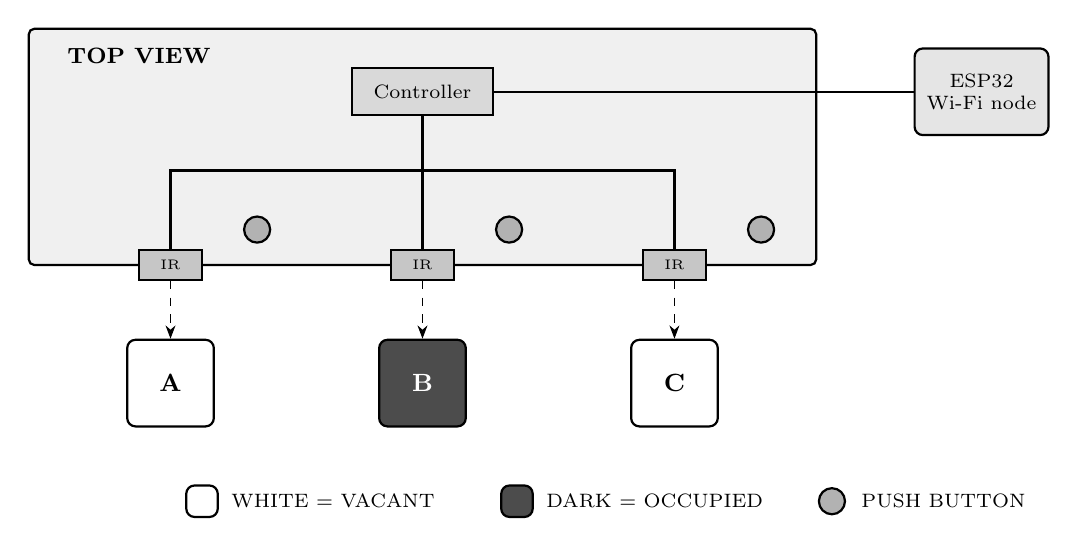
\begin{tikzpicture}[
  seat/.style={draw=black,fill=#1,thick,rounded corners=3pt,minimum size=1.1cm,font=\small\bfseries},
  irn/.style={draw,thick,fill=gray!45,minimum width=0.8cm,minimum height=0.38cm,font=\tiny}]
  \draw[thick,fill=gray!12,rounded corners=2pt] (0,0) rectangle (10,3);
  \node[font=\footnotesize\bfseries] at (1.4,2.65) {TOP VIEW};
  \node[draw,thick,fill=gray!30,minimum width=1.8cm,minimum height=0.6cm,font=\scriptsize] (ctl) at (5,2.2) {Controller};
  \foreach \x/\n in {1.8/1,5/2,8.2/3}{
    \node[irn] (ir\n) at (\x,0) {IR};
  }
  \coordinate (j) at (5,1.2);
  \draw[thick] (ctl.south) -- (j);
  \draw[thick] (j) -| (ir1.north);
  \draw[thick] (j) -- (ir2.north);
  \draw[thick] (j) -| (ir3.north);
  \node[seat=white] (c1) at (1.8,-1.5) {A};
  \node[seat=black!70,text=white] (c2) at (5.0,-1.5) {B};
  \node[seat=white] (c3) at (8.2,-1.5) {C};
  \foreach \x in {2.9,6.1,9.3}{ \node[draw,thick,fill=gray!60,circle,minimum size=0.3cm] at (\x,0.45) {}; }
  \foreach \n in {1,2,3}{ \draw[dashed,->] (ir\n.south) -- (c\n.north); }
  \node[draw,thick,fill=gray!20,rounded corners=3pt,minimum width=1.7cm,minimum height=1.1cm,
        font=\scriptsize,align=center] (wifi) at (12.1,2.2) {ESP32\\Wi-Fi node};
  \draw[thick] (ctl.east) -- (wifi.west);
  \node[seat=white,minimum size=0.4cm] at (2.2,-3.0) {};
  \node[font=\scriptsize,right] at (2.45,-3.0) {WHITE = VACANT};
  \node[seat=black!70,minimum size=0.4cm] at (6.2,-3.0) {};
  \node[font=\scriptsize,right] at (6.45,-3.0) {DARK = OCCUPIED};
  \node[draw,thick,fill=gray!60,circle,minimum size=0.3cm] at (10.2,-3.0) {};
  \node[font=\scriptsize,right] at (10.45,-3.0) {PUSH BUTTON};
\end{tikzpicture}}
\caption{Seating layout (top view): per-seat IR sensors and push buttons wired to a controller and an ESP32 node}
\label{fig:seating}
\end{figure}

\subsection{Technical Stack}
\label{sec:stack}

\begin{itemize}
  \item \textbf{Hardware:} ESP32 development board~\cite{esp32}; one IR proximity sensor per
    seat (GPIO~22, 23 and 15); one push button per seat (GPIO~25, 33 and 32) with an external
    pull-down resistor; a 5\,V power supply; perforated board and jumper wires.
  \item \textbf{Framework/Language:} C++ with the Arduino framework for the ESP32 firmware;
    JavaScript with Next.js and React for the web app~\cite{nextjs,react}, styled with
    Tailwind CSS; Node.js for the session recorder.
  \item \textbf{Database:} Firebase Realtime Database~\cite{firebase} for live seat values,
    kept under \texttt{sensors} as \texttt{ir1}, \texttt{ir2} and \texttt{ir3}, each holding
    0 (free), 1 (taken) or 2 (reserved). Cloud Firestore~\cite{firestore} for reservations,
    sessions, opening hours, students and staff.
  \item \textbf{Libraries:} the ESP32 \texttt{WiFi} and \texttt{Firebase\_ESP\_Client}
    libraries; the Firebase SDK in the web app for live updates and staff sign-in; Firebase
    Admin on the server for reservations and settings; Recharts for the charts.
  \item \textbf{Tools:} an Arduino-compatible IDE to build and upload the firmware; Git for
    version control; Vercel to host the web app~\cite{vercel}; a web browser on a laptop, a
    tablet and a phone for testing the dashboards.
\end{itemize}

\section{System Modeling Diagrams}
\label{sec:models}

Each diagram shows the system from a different angle: who uses it (use case), how data
moves (DFDs), what happens over time (sequence diagram and state machine) and the order of
steps in the firmware (flowchart).

\subsection{Use Case Diagram}

Figure~\ref{fig:usecase} shows who uses the system and how~\cite{uml}. Users view the seat
map and availability and reserve seats, staff view the reports and set opening hours, the
sensor node detects seats and sends their values, and the recorder saves sessions.

\begin{figure}[H]
\centering
\fitfig[0.42]{%
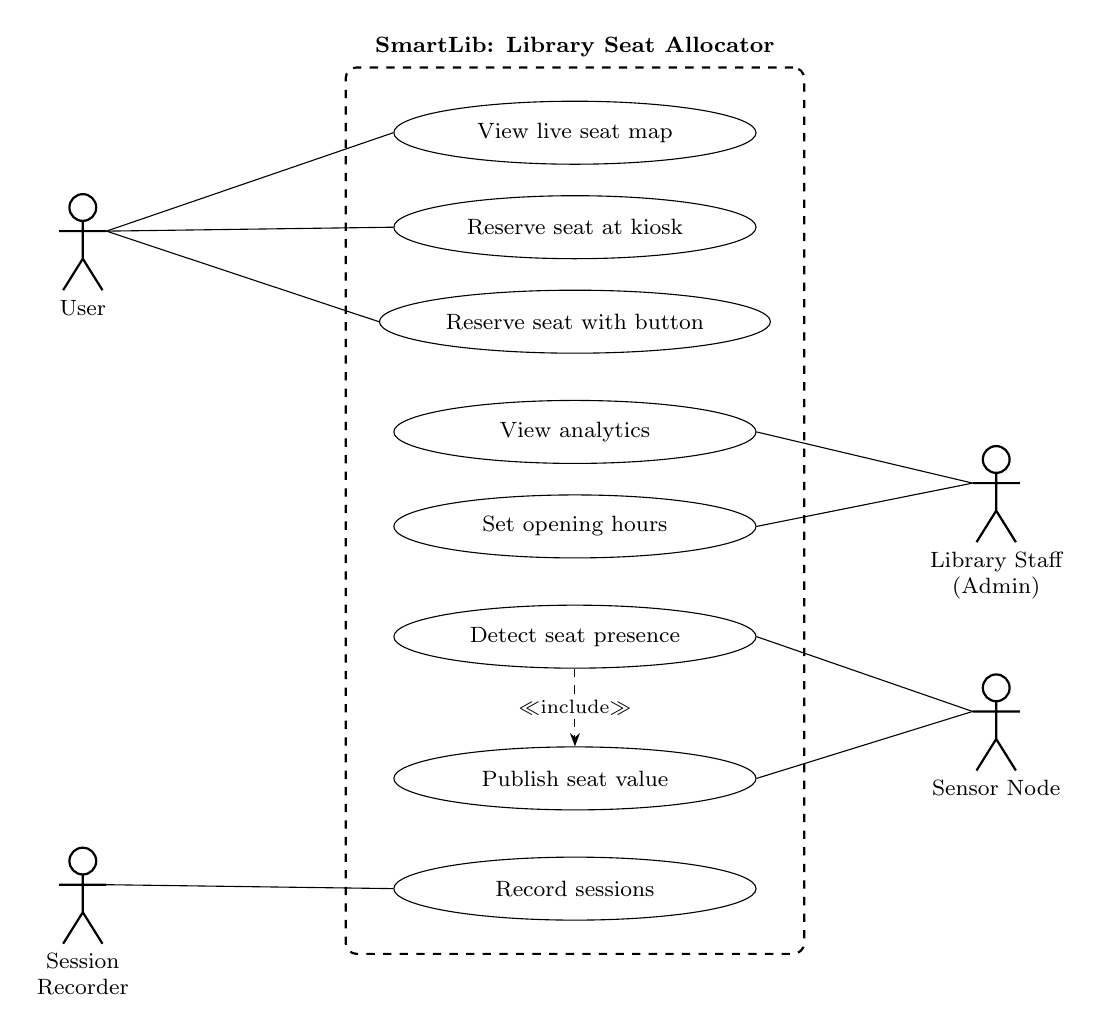
\begin{tikzpicture}[
  uc/.style={ellipse,draw,fill=white,minimum height=0.8cm,minimum width=4.6cm,align=center,font=\footnotesize}]
  \node[uc] (uc1) at (6.25,4.2)  {View live seat map};
  \node[uc] (uc2) at (6.25,3.0)  {Reserve seat at kiosk};
  \node[uc] (uc3) at (6.25,1.8)  {Reserve seat with button};
  \node[uc] (uc4) at (6.25,0.4)  {View analytics};
  \node[uc] (uc5) at (6.25,-0.8) {Set opening hours};
  \node[uc] (uc6) at (6.25,-2.2) {Detect seat presence};
  \node[uc] (uc7) at (6.25,-4.0) {Publish seat value};
  \node[uc] (uc8) at (6.25,-5.4) {Record sessions};
  \node[draw,thick,dashed,rounded corners,fit=(uc1)(uc2)(uc3)(uc4)(uc5)(uc6)(uc7)(uc8),inner sep=12pt,
        label={[font=\footnotesize\bfseries]above:SmartLib: Library Seat Allocator}] (sys) {};
  \actor{0}{2.7}{User}
  \actor{11.6}{-0.5}{Library Staff\\(Admin)}
  \actor{11.6}{-3.4}{Sensor Node}
  \actor{0}{-5.6}{Session\\Recorder}
  \draw (0.3,2.95) -- (uc1.west);
  \draw (0.3,2.95) -- (uc2.west);
  \draw (0.3,2.95) -- (uc3.west);
  \draw (11.3,-0.25) -- (uc4.east);
  \draw (11.3,-0.25) -- (uc5.east);
  \draw (11.3,-3.15) -- (uc6.east);
  \draw (11.3,-3.15) -- (uc7.east);
  \draw (0.3,-5.35) -- (uc8.west);
  \draw[->,dashed] (uc6) -- node[fill=white,inner sep=1pt,font=\scriptsize]{$\ll$include$\gg$} (uc7);
\end{tikzpicture}}
\caption{Use case diagram}
\label{fig:usecase}
\end{figure}

\subsection{Data Flow Diagrams}

The level-0 diagram (Figure~\ref{fig:dfd0}) shows the whole system as one process. The
level-1 diagram (Figure~\ref{fig:dfd1}) splits it into five processes and two data stores.

\begin{figure}[H]
\centering
\fitfig[0.27]{%
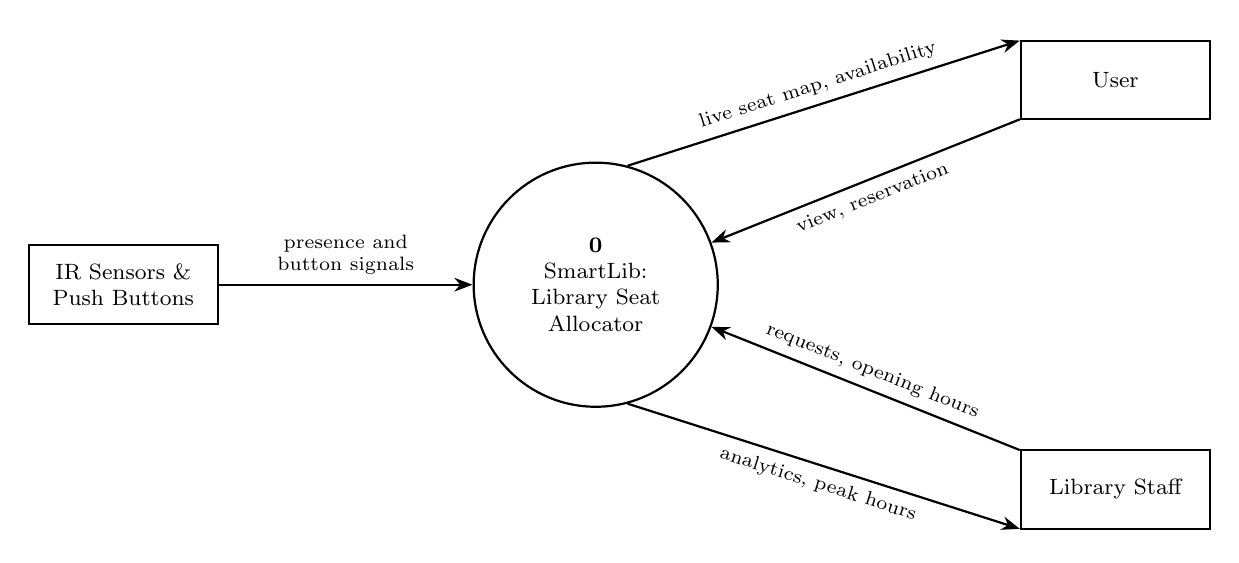
\begin{tikzpicture}[
  ent/.style={rectangle,draw,thick,fill=white,minimum width=2.4cm,minimum height=1cm,align=center,font=\footnotesize},
  proc/.style={circle,draw,thick,fill=white,minimum size=3.1cm,align=center,font=\footnotesize}]
  \node[ent]  (sens) at (0,0) {IR Sensors \&\\Push Buttons};
  \node[proc] (sys)  at (6,0) {\textbf{0}\\SmartLib:\\Library Seat\\Allocator};
  \node[ent]  (stud) at (12.6,2.6)  {User};
  \node[ent]  (adm)  at (12.6,-2.6) {Library Staff};
  \draw[->,thick] (sens) -- node[fl,above]{presence and\\button signals} (sys);
  \draw[->,thick] (sys.75) -- node[fl,above,sloped]{live seat map, availability} ([yshift=5mm]stud.west);
  \draw[->,thick] ([yshift=-5mm]stud.west) -- node[fl,below,sloped]{view, reservation} (sys.20);
  \draw[->,thick] (sys.-75) -- node[fl,below,sloped]{analytics, peak hours} ([yshift=-5mm]adm.west);
  \draw[->,thick] ([yshift=5mm]adm.west) -- node[fl,above,sloped]{requests, opening hours} (sys.-20);
\end{tikzpicture}}
\caption{Data flow diagram -- level 0 (context diagram)}
\label{fig:dfd0}
\end{figure}

\begin{figure}[H]
\centering
\fitfig[0.36]{%
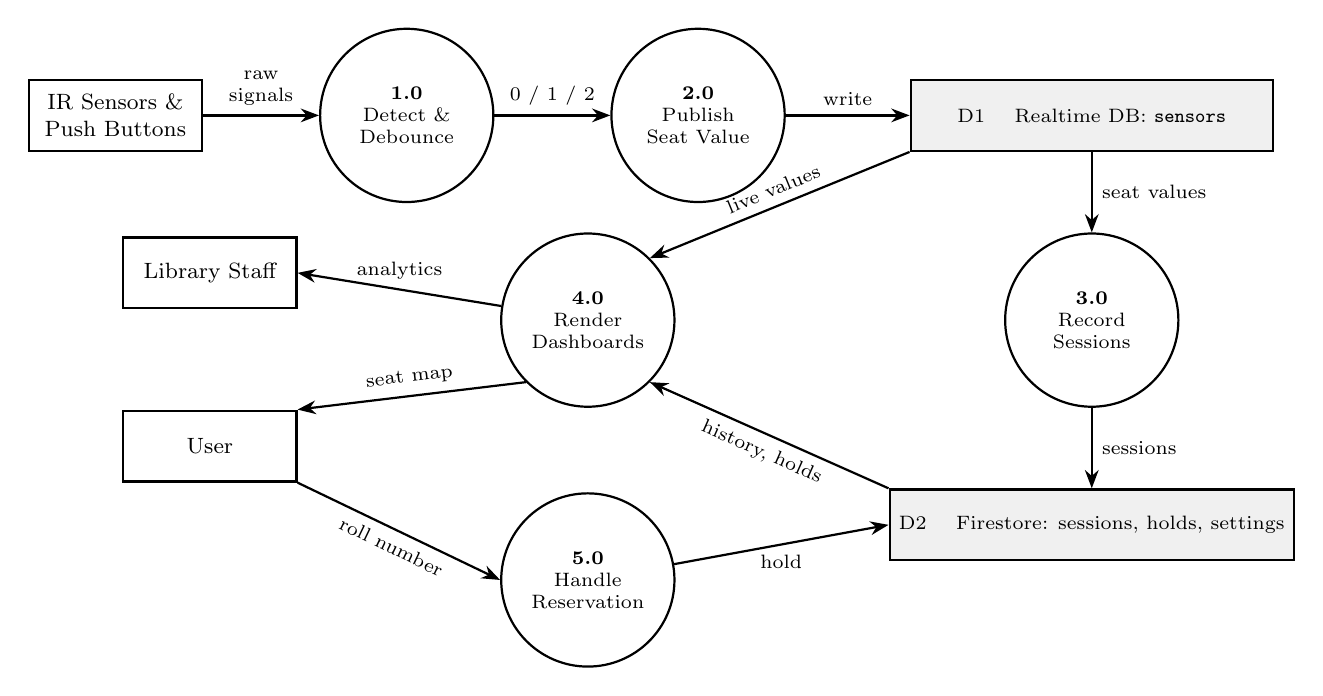
\begin{tikzpicture}[
  ent/.style={rectangle,draw,thick,fill=white,minimum width=2.2cm,minimum height=0.9cm,align=center,font=\footnotesize},
  proc/.style={circle,draw,thick,fill=white,minimum size=2.2cm,align=center,font=\scriptsize},
  store/.style={rectangle,draw,thick,fill=gray!12,minimum width=4.6cm,minimum height=0.9cm,align=center,font=\scriptsize}]
  \node[ent]  (sens) at (0,0)    {IR Sensors \&\\Push Buttons};
  \node[proc] (p1)   at (3.7,0)  {\textbf{1.0}\\Detect \&\\Debounce};
  \node[proc] (p2)   at (7.4,0)  {\textbf{2.0}\\Publish\\Seat Value};
  \node[store](d1)   at (12.4,0) {D1 \quad Realtime DB: \texttt{sensors}};
  \node[proc] (p3)   at (12.4,-2.6) {\textbf{3.0}\\Record\\Sessions};
  \node[store](d2)   at (12.4,-5.2) {D2 \quad Firestore: sessions, holds, settings};
  \node[proc] (p4)   at (6.0,-2.6) {\textbf{4.0}\\Render\\Dashboards};
  \node[proc] (p5)   at (6.0,-5.9) {\textbf{5.0}\\Handle\\Reservation};
  \node[ent]  (stud) at (1.2,-4.2)  {User};
  \node[ent]  (adm)  at (1.2,-2.0)  {Library Staff};
  \draw[->,thick] (sens) -- node[fl,above]{raw\\signals} (p1);
  \draw[->,thick] (p1) -- node[fl,above]{0 / 1 / 2} (p2);
  \draw[->,thick] (p2) -- node[fl,above]{write} (d1);
  \draw[->,thick] (d1) -- node[fl,right]{seat values} (p3);
  \draw[->,thick] (p3) -- node[fl,right]{sessions} (d2);
  \draw[->,thick] (d1.south west) -- node[fl,above,sloped]{live values} (p4.north east);
  \draw[->,thick] (d2.north west) -- node[fl,below,sloped]{history, holds} (p4.south east);
  \draw[->,thick] (p4) -- node[fl,above]{analytics} (adm.east);
  \draw[->,thick] (p4.south west) -- node[fl,above,sloped]{seat map} (stud.north east);
  \draw[->,thick] (stud.south east) -- node[fl,below,sloped]{roll number} (p5.west);
  \draw[->,thick] (p5) -- node[fl,below]{hold} (d2.west);
\end{tikzpicture}}
\caption{Data flow diagram -- level 1}
\label{fig:dfd1}
\end{figure}

\subsection{Sequence Diagram}

Figure~\ref{fig:seq} follows one event, from a user sitting down to the seat turning red on
every dashboard. The ESP32 sends the update only after the reading stays the same for
5~seconds. Figure~\ref{fig:seqkiosk} follows a reservation made at the entrance kiosk.

\begin{figure}[H]
\centering
\fitfig[0.36]{%
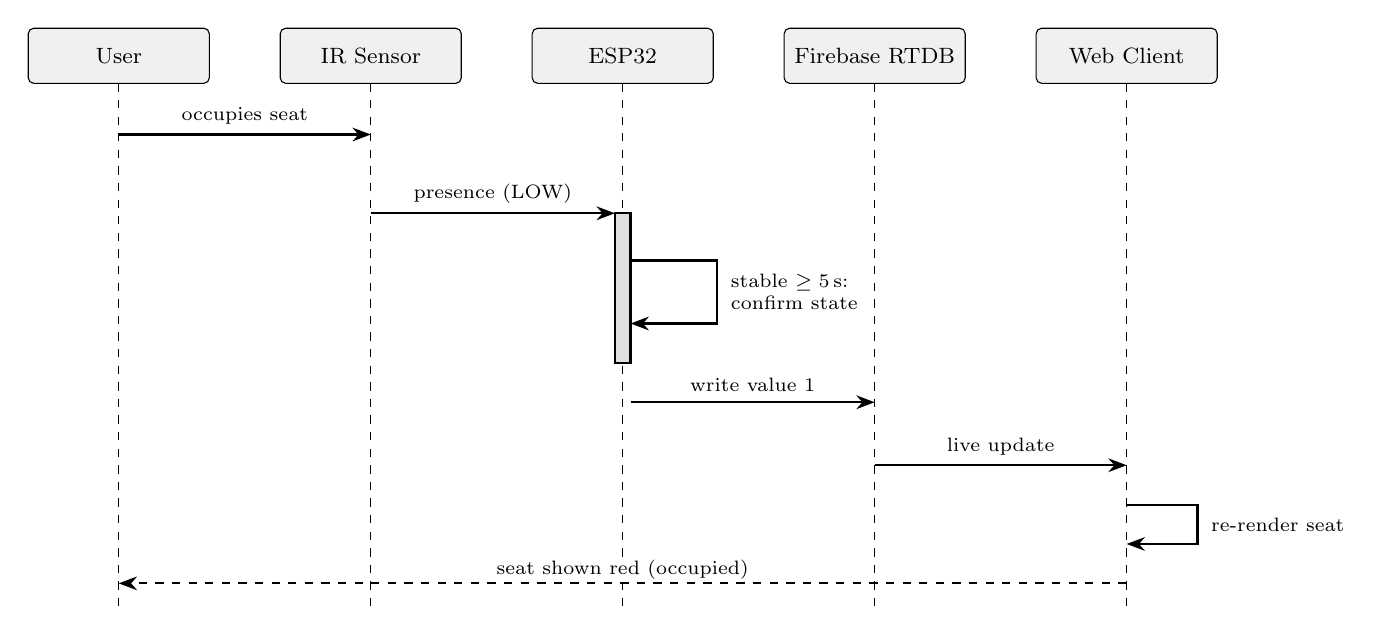
\begin{tikzpicture}[x=1cm,y=1cm]
  \foreach \x/\n in {0/User,3.2/IR Sensor,6.4/ESP32,9.6/Firebase RTDB,12.8/Web Client}{
    \node[draw,fill=gray!12,rounded corners=2pt,minimum width=2.3cm,minimum height=0.7cm,font=\footnotesize] at (\x,0) {\n};
    \draw[dashed] (\x,-0.35) -- (\x,-7.0);
  }
  % activation bar: ESP32 waiting for the debounce window
  \draw[thick,fill=gray!25] (6.3,-2.0) rectangle (6.5,-3.9);
  \draw[->,thick] (0,-1.0)   -- node[above,font=\scriptsize]{occupies seat} (3.2,-1.0);
  \draw[->,thick] (3.2,-2.0) -- node[above,font=\scriptsize]{presence (LOW)} (6.3,-2.0);
  \draw[->,thick] (6.5,-2.6) -- (7.6,-2.6) -- (7.6,-3.4) -- (6.5,-3.4);
  \node[font=\scriptsize,right,align=left] at (7.65,-3.0) {stable $\geq 5$\,s:\\confirm state};
  \draw[->,thick] (6.5,-4.4) -- node[above,font=\scriptsize]{write value 1} (9.6,-4.4);
  \draw[->,thick] (9.6,-5.2) -- node[above,font=\scriptsize]{live update} (12.8,-5.2);
  \draw[->,thick] (12.8,-5.7) -- (13.7,-5.7) -- (13.7,-6.2) -- (12.8,-6.2);
  \node[font=\scriptsize,right] at (13.75,-5.95) {re-render seat};
  \draw[->,thick,dashed] (12.8,-6.7) -- node[above,font=\scriptsize,fill=white,inner sep=1pt]{seat shown red (occupied)} (0,-6.7);
\end{tikzpicture}}
\caption{Sequence diagram for a seat-occupancy event, including the 5-second debounce}
\label{fig:seq}
\end{figure}

\begin{figure}[H]
\centering
\fitfig[0.36]{%
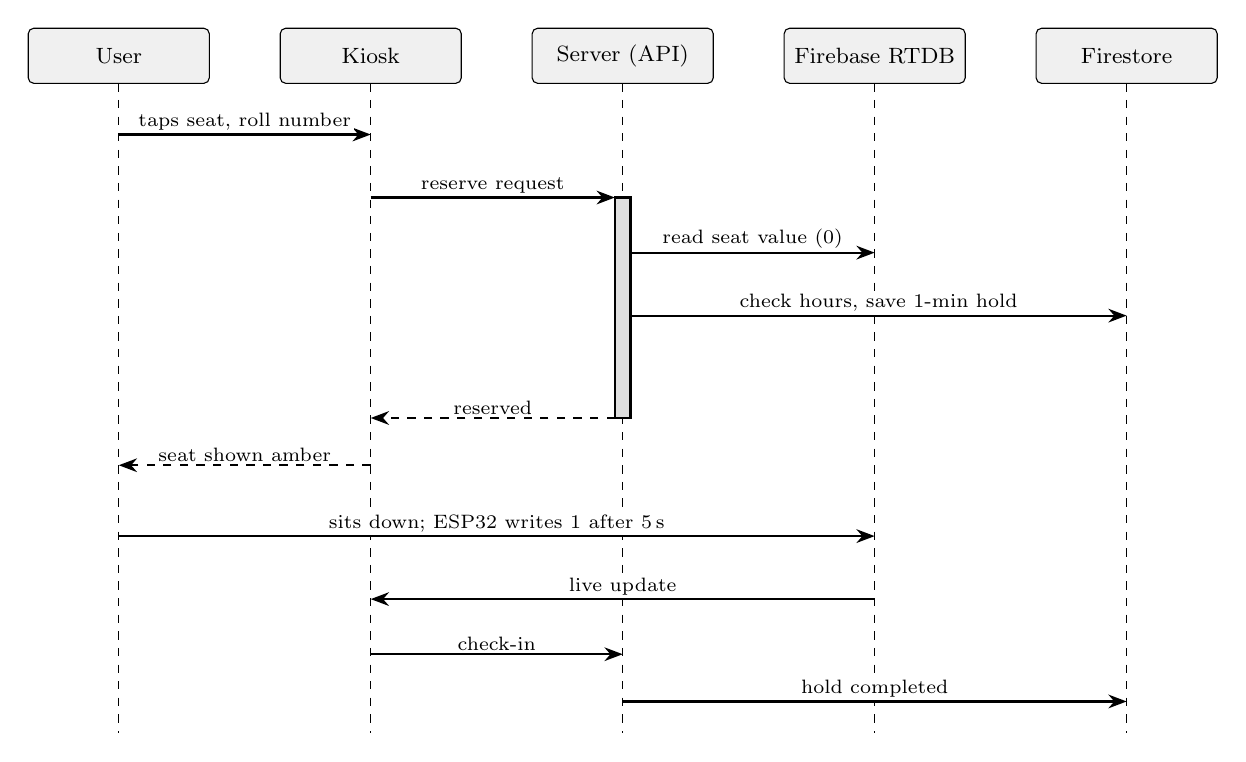
\begin{tikzpicture}[x=1cm,y=1cm]
  \foreach \x/\n in {0/User,3.2/Kiosk,6.4/Server (API),9.6/Firebase RTDB,12.8/Firestore}{
    \node[draw,fill=gray!12,rounded corners=2pt,minimum width=2.3cm,minimum height=0.7cm,font=\footnotesize] at (\x,0) {\n};
    \draw[dashed] (\x,-0.35) -- (\x,-8.6);
  }
  \draw[thick,fill=gray!25] (6.3,-1.8) rectangle (6.5,-4.6);
  \draw[->,thick] (0,-1.0)   -- node[above,font=\scriptsize,fill=white,inner sep=1pt]{taps seat, roll number} (3.2,-1.0);
  \draw[->,thick] (3.2,-1.8) -- node[above,font=\scriptsize,fill=white,inner sep=1pt]{reserve request} (6.3,-1.8);
  \draw[->,thick] (6.5,-2.5) -- node[above,font=\scriptsize,fill=white,inner sep=1pt]{read seat value (0)} (9.6,-2.5);
  \draw[->,thick] (6.5,-3.3) -- node[above,font=\scriptsize,fill=white,inner sep=1pt]{check hours, save 1-min hold} (12.8,-3.3);
  \draw[->,thick,dashed] (6.3,-4.6) -- node[above,font=\scriptsize,fill=white,inner sep=1pt]{reserved} (3.2,-4.6);
  \draw[->,thick,dashed] (3.2,-5.2) -- node[above,font=\scriptsize,fill=white,inner sep=1pt]{seat shown amber} (0,-5.2);
  \draw[->,thick] (0,-6.1)   -- node[above,font=\scriptsize,fill=white,inner sep=1pt]{sits down; ESP32 writes 1 after 5\,s} (9.6,-6.1);
  \draw[->,thick] (9.6,-6.9) -- node[above,font=\scriptsize,fill=white,inner sep=1pt]{live update} (3.2,-6.9);
  \draw[->,thick] (3.2,-7.6) -- node[above,font=\scriptsize,fill=white,inner sep=1pt]{check-in} (6.4,-7.6);
  \draw[->,thick] (6.4,-8.2) -- node[above,font=\scriptsize,fill=white,inner sep=1pt]{hold completed} (12.8,-8.2);
\end{tikzpicture}}
\caption{Sequence diagram for a kiosk reservation and check-in}
\label{fig:seqkiosk}
\end{figure}

\subsection{Seat State Machine}

Each seat follows the three states in Figure~\ref{fig:fsm}, which match the values sent to
the database: \textsc{Free} (0), \textsc{Occupied} (1) and \textsc{Reserved} (2). A change
between free and occupied is sent only when the new reading holds for 5~seconds; a shorter
change (dashed arrows) is ignored. Holding the push button for 3~seconds reserves the seat
for 60~seconds, after which the ESP32 returns it to the current sensor reading. A kiosk
reservation is kept only in the web app: the seat value stays 0 and the app shows it as
reserved until the hold ends or the seat becomes occupied.

\begin{figure}[H]
\centering
\fitfig[0.36]{%
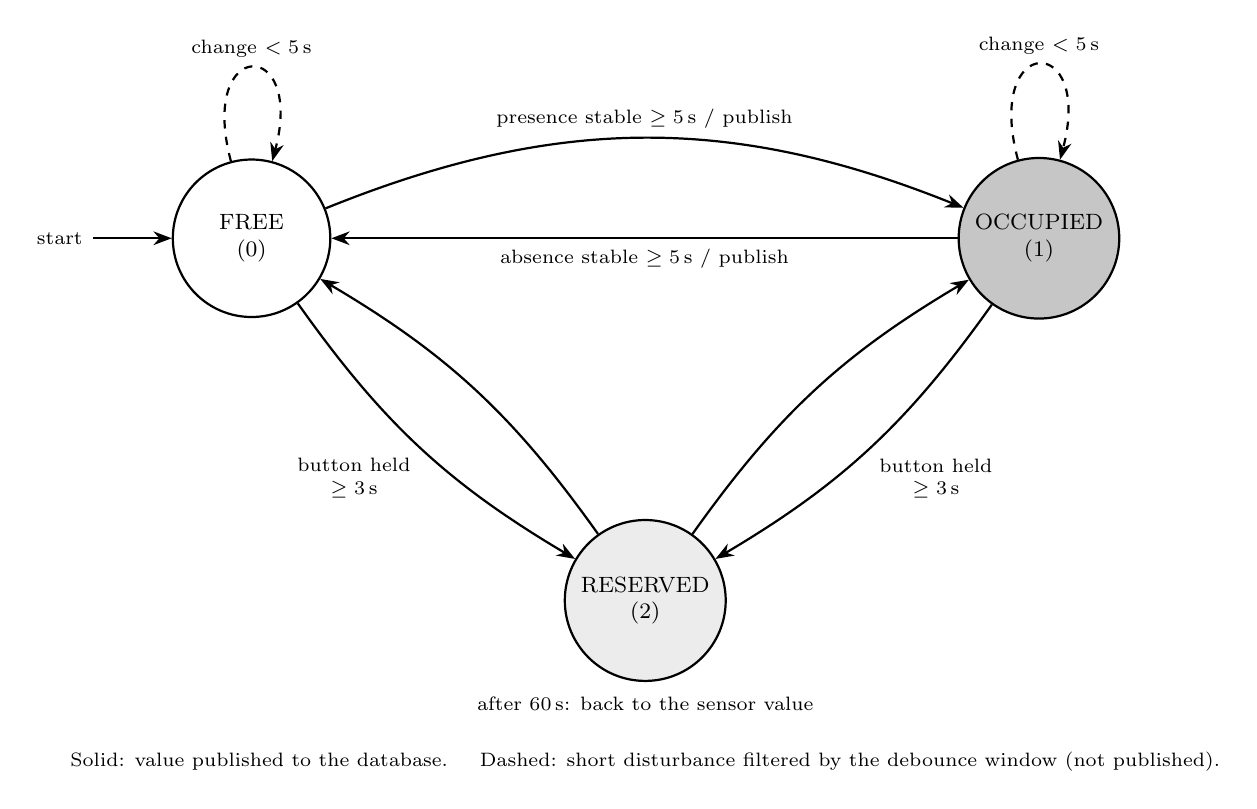
\begin{tikzpicture}[
  st/.style={circle,draw,thick,minimum size=2.0cm,align=center,font=\footnotesize}]
  \node[st,fill=white]   (v)  at (0,0)    {FREE\\(0)};
  \node[st,fill=gray!45] (o)  at (10,0)   {OCCUPIED\\(1)};
  \node[st,fill=gray!15] (r)  at (5,-4.6) {RESERVED\\(2)};
  \draw[<-,thick] (v.west) -- ++(-1.0,0) node[fl,left]{start};
  \draw[->,thick] (v)  to[bend left=22]  node[fl,above]{presence stable $\geq 5$\,s / publish} (o);
  \draw[->,thick] (o)  -- node[fl,below]{absence stable $\geq 5$\,s / publish} (v);
  \draw[->,thick] (v)  to[bend right=12] node[fl,below left]{button held\\$\geq 3$\,s} (r);
  \draw[->,thick] (o)  to[bend left=12]  node[fl,below right]{button held\\$\geq 3$\,s} (r);
  \draw[->,thick] (r)  to[bend right=12] (v);
  \draw[->,thick] (r)  to[bend left=12]  (o);
  \node[fl,anchor=north] at (5,-5.7) {after 60\,s: back to the sensor value};
  \draw[->,thick,dashed] (v) to[loop above] node[fl,above]{change $<5$\,s} (v);
  \draw[->,thick,dashed] (o) to[loop above] node[fl,above]{change $<5$\,s} (o);
  \node[fl,anchor=north] at (5,-6.4) {Solid: value published to the database. \quad
        Dashed: short disturbance filtered by the debounce window (not published).};
\end{tikzpicture}}
\caption{Seat state machine with 5-second debounce and 60-second button reservation}
\label{fig:fsm}
\end{figure}

\subsection{ESP32 Firmware Flowchart}

Figure~\ref{fig:flow} shows the order of steps in the firmware. After start-up, the loop
reads each button and sensor. A button held for 3~seconds sets the seat to 2 for 60~seconds.
Otherwise the seat follows its sensor once the reading has held for 5~seconds, and a value is
sent only when it changes. The state machine describes one seat; the flowchart describes the
program.

\begin{figure}[H]
\centering
\fitfig[0.42]{%
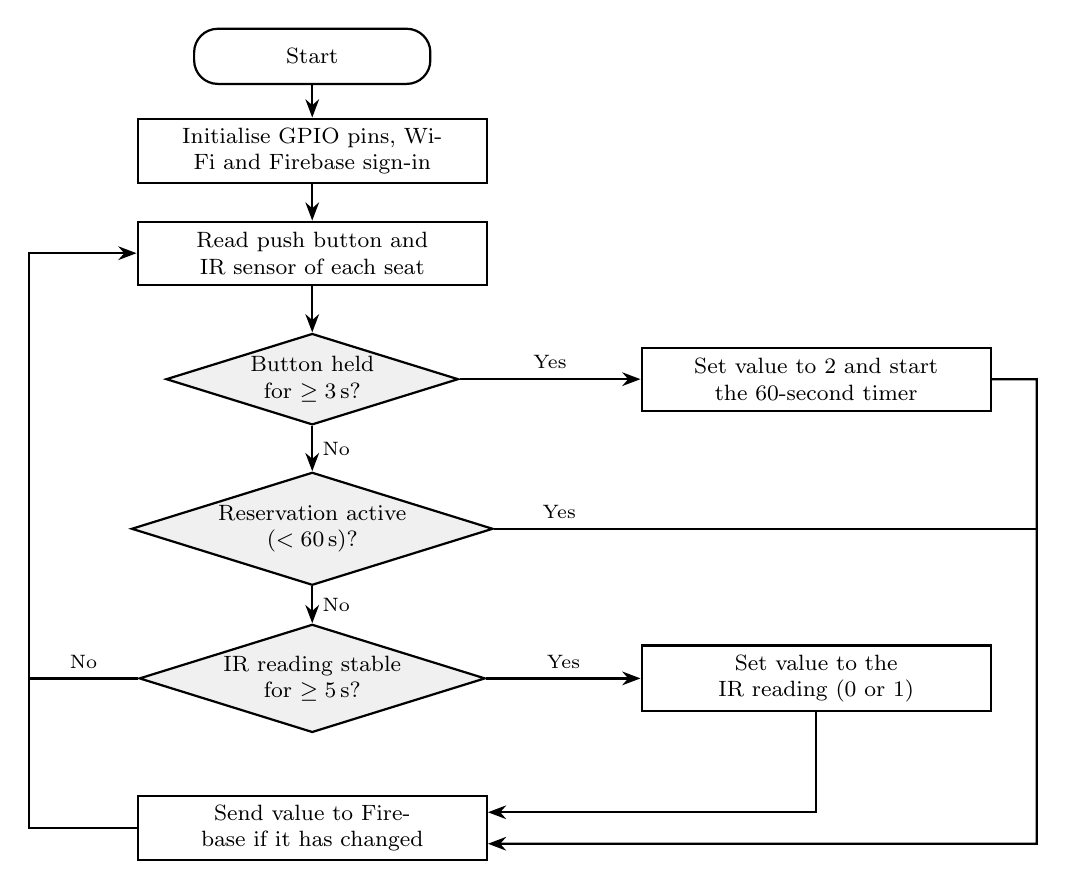
\begin{tikzpicture}[
  term/.style={rectangle,rounded corners=0.3cm,draw,thick,fill=white,minimum height=0.7cm,minimum width=3cm,font=\footnotesize,align=center},
  prc/.style={rectangle,draw,thick,fill=white,minimum height=0.8cm,text width=4.2cm,font=\footnotesize,align=center},
  dec/.style={diamond,aspect=3.2,draw,thick,fill=gray!12,inner sep=1pt,font=\footnotesize,align=center}]
  \node[term] (start) at (0,0)    {Start};
  \node[prc]  (init)  at (0,-1.2) {Initialise GPIO pins, Wi-Fi and Firebase sign-in};
  \node[prc]  (read)  at (0,-2.5) {Read push button and IR sensor of each seat};
  \node[dec]  (d1)    at (0,-4.1) {Button held\\for $\geq 3$\,s?};
  \node[dec]  (d2)    at (0,-6.0) {Reservation active\\($<60$\,s)?};
  \node[dec]  (d3)    at (0,-7.9) {IR reading stable\\for $\geq 5$\,s?};
  \node[prc]  (b1)    at (6.4,-4.1) {Set value to 2 and start the 60-second timer};
  \node[prc]  (upd)   at (6.4,-7.9) {Set value to the IR reading (0 or 1)};
  \node[prc]  (send)  at (0,-9.8) {Send value to Firebase if it has changed};
  \draw[->,thick] (start) -- (init);
  \draw[->,thick] (init) -- (read);
  \draw[->,thick] (read) -- (d1);
  \draw[->,thick] (d1) -- node[right,font=\scriptsize]{No} (d2);
  \draw[->,thick] (d1) -- node[above,font=\scriptsize]{Yes} (b1);
  \draw[->,thick] (b1.east) -- (9.2,-4.1) -- (9.2,-10.0) -- ([yshift=-2mm]send.east);
  \draw[thick] (d2.east) -- node[above,font=\scriptsize,pos=0.12]{Yes} (9.2,-6.0);
  \draw[->,thick] (d2) -- node[right,font=\scriptsize]{No} (d3);
  \draw[->,thick] (d3) -- node[above,font=\scriptsize]{Yes} (upd);
  \draw[->,thick] (upd.south) |- ([yshift=2mm]send.east);
  \draw[->,thick] (send.west) -- (-3.6,-9.8) -- (-3.6,-2.5) -- (read.west);
  \draw[thick] (d3.west) -- node[above,font=\scriptsize]{No} (-3.6,-7.9);
\end{tikzpicture}}
\caption{Firmware main-loop flowchart}
\label{fig:flow}
\end{figure}

\section{Implementation Details}

\subsection{Firmware (ESP32)}
% (ESP32)}

The firmware reads the IR pins and push buttons, applies the 5-second debounce to each seat,
handles the 60-second button reservation and writes the seat value to the database.
Listing~\ref{lst:fw} shows this logic; pin numbers match Section~\ref{sec:stack}. The Wi-Fi
and Firebase passwords are kept in a separate file that is not stored in the code repository.

\Needspace{30\baselineskip}
\begin{lstlisting}[style=code,language=C++,caption={Illustrative firmware logic for debounce, reservation and publishing},label={lst:fw}]
constexpr uint32_t IR_DEBOUNCE_MS = 5000;  // 5-second debounce window
constexpr uint32_t BUTTON_HOLD_MS = 3000;  // hold button for 3 s
constexpr uint32_t RESERVE_MS     = 60000; // reservation lasts 60 s
const uint8_t irPins[3]  = {22, 23, 15};
const uint8_t btnPins[3] = {25, 33, 32};
const char* paths[3] = {"/sensors/ir1", "/sensors/ir2", "/sensors/ir3"};

void updateSeat(int i, uint32_t now) {
  int raw = (digitalRead(irPins[i]) == LOW) ? 1 : 0;   // active-low IR
  if (raw != rawIR[i]) { rawIR[i] = raw; changedAt[i] = now; }
  if (raw != stableIR[i] && now - changedAt[i] >= IR_DEBOUNCE_MS)
    stableIR[i] = raw;                                  // confirmed 0 or 1
  if (buttonHeldFor(i, now) >= BUTTON_HOLD_MS && !reserved[i]) {
    reserved[i] = true;  reservedAt[i] = now;           // start reservation
  }
  if (reserved[i] && now - reservedAt[i] >= RESERVE_MS)
    reserved[i] = false;                                // back to sensor
  desired[i] = reserved[i] ? 2 : stableIR[i];
}
void loop() {
  uint32_t now = millis();
  for (int i = 0; i < 3; ++i) {
    updateSeat(i, now);
    if (desired[i] != sent[i] &&
        Firebase.RTDB.setInt(&fbdo, paths[i], desired[i]))
      sent[i] = desired[i];                             // write only on change
  }
}
\end{lstlisting}

\subsection{Cloud Layer and Web Application}

The Firebase Realtime Database holds the seat values described in Section~\ref{sec:stack}.
The web app listens to the database and receives each change over an open connection, so it
never needs to ask for updates. Its database rules let everyone read the seat values but only
the signed-in ESP32 account write them, and only as a number from 0 to 2. Cloud Firestore
holds the reservations, sessions, opening hours, students and staff.

\textbf{Data and server routes.}
\begin{itemize}
  \item \texttt{sensors/ir1}--\texttt{ir3} (Realtime Database): one value per seat, written
    only by the ESP32.
  \item Firestore: \texttt{holds} and \texttt{reservations} for kiosk bookings,
    \texttt{sessions} for usage history, \texttt{config/settings} for opening hours, and
    \texttt{students} and \texttt{admins} for sign-in checks.
  \item \texttt{/api/reserve} checks the seat value, opening hours and the one-hold rule
    before saving a hold; \texttt{/api/checkin} completes a hold once its seat reads 1;
    \texttt{/api/settings} lets signed-in staff save opening hours.
\end{itemize}

The web app, called \emph{SmartLib}, is built with Next.js and React~\cite{nextjs,react} and
runs online on Vercel~\cite{vercel}. The status of each seat is never stored; the app works it
out from the seat value, any kiosk hold and the opening hours, as \emph{Available},
\emph{Occupied}, \emph{Reserved}, \emph{Closed} or \emph{Unavailable}. A seat under
maintenance or without a sensor is shown as unavailable to staff only and is left out of the
counts.

\textbf{User dashboard.} Cards show total, taken, reserved and free seats and the percentage
in use. A seat map shows the seats with free seats in green, taken seats in red and reserved
seats in amber. The header shows the time, the date, whether the library is open and the
opening hours for the week. Charts show the user's view of usage over the last 30 days.

\textbf{Admin dashboard.} Staff sign in with Google or e-mail; the sign-in lasts 7 days.
Cards show total seats, taken seats, average session time and the busiest hour. Charts show
the daily trend, hourly usage and the taken/free split for today, the last 7 days or the last
30 days, each with a one-line description. Other pages list the reservations and sessions,
show reservation activity as notifications and let staff set the opening hours for each day.

\textbf{Entrance kiosk.} A large-screen page at the library gate shows live seat
availability. A user taps a free seat and enters a roll number. The server checks that the
seat value is 0, the library is open and the user has no other active hold, then saves a
1-minute hold. When the seat becomes occupied, any open page asks the server to check the
user in, which completes the hold. The kiosk shows clear messages when the library is closed,
all seats are taken or the system cannot be reached.

\textbf{Session recorder.} The free Firebase plan does not allow server functions, so a small
Node.js program runs on a library computer. It watches the seat values and saves a session
each time a seat goes from free to occupied and back, with breaks recorded while the value is
2. Sittings shorter than 2~minutes are ignored, and a 2-minute grace period stops a short
absence from splitting a session. These sessions feed the admin charts.

\textbf{Saving database reads.} To stay within the free plan, the app keeps a local copy of
the data in the browser, loads only the last 30 days of history and does not load history on
the kiosk.

% ===== CHAPTER 3: RESULTS & EVALUATION =====

\chapter{Results and Evaluation}
\label{ch:results}

\section{Testing Methodology}

The tests in Table~\ref{tab:tests} check the requirements from Chapter~\ref{ch:method}.
They were run on the three-seat set-up with the web app online, using a laptop, a tablet and
a phone.

\begin{table}[H]
\centering
\small
\renewcommand{\arraystretch}{1.1}
\begin{tabularx}{\linewidth}{|l|>{\raggedright\arraybackslash}p{0.3\linewidth}|>{\raggedright\arraybackslash}X|>{\raggedright\arraybackslash}p{0.19\linewidth}|}
  \hline
  \textbf{ID} & \textbf{Scenario} & \textbf{Expected outcome} & \textbf{Req.} \\
  \hline
  T1 & A person sits in a free seat & After 5\,s the seat turns red on all dashboards
       & FR1, FR2, FR4 \\
  \hline
  T2 & The person leaves the seat & After 5\,s the seat turns green & FR1, FR2, FR4 \\
  \hline
  T3 & A hand passes the sensor for less than 5\,s & No change is sent & FR2, NFR2 \\
  \hline
  T4 & Two screens are open at once & Both update together without a refresh
       & FR4, NFR1 \\
  \hline
  T5 & The push button is held for 3\,s & The seat turns amber for 60\,s & FR3, FR5 \\
  \hline
  T6 & A free seat is reserved at the kiosk & The seat turns amber; the hold ends after
       1~minute if nobody sits & FR6 \\
  \hline
  T7 & The user sits in the reserved seat & The hold is completed and the seat turns red
       & FR6 \\
  \hline
  T8 & The same roll number reserves a second seat & The kiosk refuses the request & FR6 \\
  \hline
  T9 & A person sits for more than 2~minutes & One session is saved and shown in the
       charts & FR7 \\
  \hline
  T10 & The library is closed & Seats show as closed and the kiosk takes no reservations
        & FR8 \\
  \hline
  T11 & The admin page is opened without signing in & The sign-in page is shown & NFR4 \\
  \hline
\end{tabularx}
\caption{Test cases and expected outcomes}
\label{tab:tests}
\end{table}

\section{Analysis}

The system shows the full path: IR sensor to ESP32, ESP32 to the cloud database, and
database to live browser dashboards. Sensing each seat fixes the main weakness of gate
counters, and the 5-second debounce keeps seat colours steady. Keeping the hardware as the
only writer of seat values, and doing reservations, sessions and opening hours in software,
meant the firmware did not need to change as features were added.

Testing found several problems that were then fixed. A kiosk-reserved seat stayed reserved
after the user sat down and left, so a check-in step was added that completes the hold as soon
as the seat is taken. The online server failed on reservations because of a library that
needed a newer Node.js version, so the version was fixed. The free plan's daily read limit was
reached during testing, so the app now keeps a local copy of the data, loads less history and
shows a clear message instead of waiting without end.

\subsection{Limitations}

An IR sensor detects any object, not only a person, so a bag left on a desk shows the seat
as taken. The system needs library Wi-Fi and the cloud service, and larger set-ups need more
nodes, careful wiring and power planning, and sensor tuning. The session recorder must be
running on a library computer for usage history to be saved, and the free Firebase plan limits
how many times the data can be read each day. The kiosk accepts any roll number in the
student list and does not check an ID card.

% ===== CHAPTER 4: CONCLUSION =====

\chapter{Conclusion}
\label{ch:concl}

\section{Summary of Work}

This project builds SmartLib, a real-time Library Seat Allocator, from low-cost IoT hardware and a cloud
database. It solves the three problems found earlier: users can see free seats before
walking in, each desk's status is shown instead of a total count, and staff get live and past
usage data. The final system adds short reservations from the desk button and the entrance
kiosk, session history for the charts, staff-set opening hours and a secure admin sign-in,
and runs online so it can be opened on any phone or screen.

\section{Future Work and Recommendations}

\begin{enumerate}
  \item Add a second type of sensor to tell a person apart from an object.
  \item Check the user's ID card at the kiosk with an RFID or barcode reader.
  \item Move the session recorder to a cloud function so no library computer is needed.
  \item Use past data to predict busy hours.
  \item Use a lighter messaging method such as MQTT, and battery or low-power operation.
  \item Cover more zones and floors with a campus-wide map.
  \item Send alerts when a chosen seat or zone becomes free.
\end{enumerate}

% ===== BIBLIOGRAPHY =====

% Entries not cited in the text are still listed
\nocite{pressman,sommerville}

\clearpage
\phantomsection
\addcontentsline{toc}{chapter}{Bibliography}
\begin{thebibliography}{BRJ05}
\bibitem[BRJ05]{uml} Grady Booch, James Rumbaugh, and Ivar Jacobson. \emph{The Unified Modeling Language User Guide}. 2nd ed. Addison-Wesley, 2005.
\bibitem[Esp]{esp32} Espressif Systems. \emph{ESP32 Series Datasheet}. Espressif Systems. \url{https://www.espressif.com}.
\bibitem[Goo]{firebase} Google. \emph{Firebase Realtime Database Documentation}. \url{https://firebase.google.com/docs/database}.
\bibitem[Goo]{firestore} Google. \emph{Cloud Firestore Documentation}. \url{https://firebase.google.com/docs/firestore}.
\bibitem[Met]{react} Meta Open Source. \emph{React Documentation}. \url{https://react.dev}.
\bibitem[Ver]{nextjs} Vercel. \emph{Next.js Documentation}. \url{https://nextjs.org/docs}.
\bibitem[Ver]{vercel} Vercel. \emph{Vercel Documentation}. \url{https://vercel.com/docs}.
\bibitem[PM19]{pressman} Roger S. Pressman and Bruce R. Maxim. \emph{Software Engineering: A Practitioner's Approach}. 9th ed. McGraw-Hill, 2019.
\bibitem[Som16]{sommerville} Ian Sommerville. \emph{Software Engineering}. 10th ed. Pearson, 2016.
\end{thebibliography}

\end{document}
